%%%%%%%%%%%%%%%%%%%%%%%%%%%%%%%%%%%%%%%%%
% University/School Laboratory Report
% LaTeX Template
% Version 3.1 (25/3/14)
%
% This template has been downloaded from:
% http://www.LaTeXTemplates.com
%
% Original author:
% Linux and Unix Users Group at Virginia Tech Wiki 
% (https://vtluug.org/wiki/Example_LaTeX_chem_lab_report)
%
% License:
% CC BY-NC-SA 3.0 (http://creativecommons.org/licenses/by-nc-sa/3.0/)
%
%%%%%%%%%%%%%%%%%%%%%%%%%%%%%%%%%%%%%%%%%

%----------------------------------------------------------------------------------------
%	PACKAGES AND DOCUMENT CONFIGURATIONS
%----------------------------------------------------------------------------------------

\documentclass{article}

\usepackage[version=3]{mhchem} % Package for chemical equation typesetting
\usepackage{siunitx} % Provides the \SI{}{} and \si{} command for typesetting SI units
\usepackage{graphicx} % Required for the inclusion of images
\usepackage{natbib} % Required to change bibliography style to APA
\usepackage{amsmath} % Required for some math elements 
\usepackage{todonotes}
\usepackage{wrapfig}
\usepackage{caption}
%\usepackage{chemmacros}
\usepackage[export]{adjustbox}
\usepackage{pbox}
\usepackage{listings}
\lstset{
captionpos=b,
language=c,
stepnumber=2,
tabsize=2,
frame=single,
label=DescriptiveLabel,
% upquote=true,
aboveskip={1.5\baselineskip},
columns=fullflexible,
showstringspaces=false,
extendedchars=true,
breaklines=true,
showtabs=false,
showspaces=false,
showstringspaces=false,
% identifierstyle=\ttfamily,
% keywordstyle=\footnotesize,
% keywordstyle=\font\ttfamily,
% keywordstyle=\color[rgb]{0,0,1},
% commentstyle=\color[rgb]{0.133,0.545,0.133},
% stringstyle=\color[rgb]{0.627,0.126,0.941},
% basicstyle=\color[rgb]{0,0,0},
basicstyle=\footnotesize,
}
\usepackage{geometry}
\newgeometry{left=2cm, right=2cm, bottom=2cm, top=3cm}
\setlength\parindent{0pt} % Removes all indentation from paragraphs

\renewcommand{\labelenumi}{\alph{enumi}.} % Make numbering in the enumerate environment by letter rather than number (e.g. section 6)

%\usepackage{times} % Uncomment to use the Times New Roman font

%----------------------------------------------------------------------------------------
%	DOCUMENT INFORMATION
%----------------------------------------------------------------------------------------

% \title{Energy Aware Software} % Title

% \author{\textbf{Principal investigator}: Simon Holmbacka\\ \AA{}bo Akademi University, Embedded Systems Laboratory} % Author name

\begin{document}
\huge{Utilization of Multi-Dimensional Data for Mobile Network Performance Management\\\large{Project proposal}}
% \normalsize\textbf{Principal investigator}: Dr. Simon Holmbacka\\ 
% \textbf{Project starting time}: 01.09.2017\\
% \textbf{Duration of the project}: 48 months\\
% \textbf{Site of research}:\\
% \textit{\AA{}bo Akademi University} \\
% \textit{Faculty of Science and Engineering}\\
% \textit{Embedded Systems Laboratory}\\
% \textit{Vattenborgsv\"{a}gen 5 20500 Turku, Finland}\\

\begin{table}[h]

\normalsize\textbf{Principal investigator}: Dr. Simon Holmbacka\\
\textbf{Host university}: \AA{}bo Akademi University\\
\textbf{Duration of the project}: 24 months\\
\textbf{Site of research}:\textit{ Elisa OYJ, Helsinki, Finland}\\
\textbf{Contact person on site}: \textit{Jonas Kronlund}

\end{table}

\date{\today} % Date for the report

% \maketitle % Insert the title, author and date
\normalsize
\section{Rationale}
\label{sec:rationale}
With the exploding market in mobile telecommunication containing increased usage of social media, increased demand in bandwidth and the future of smart devices, the telecommunications industry is facing a challenge in meeting the ever increasing demand in user satisfaction.
The current standards such as 3G and 4G contains large data streams in the telecommunications network, and handling such streams efficiently is a many-parameter optimization problem.
The latest communication standard to appear on the market is the 5G mobile network, which has higher potential capacity than the previous generation networks, it is planned to handle a significantly larger amount of users for longer time intervals and a latency of 1ms is targeted.
To reach sufficient performance in current network standards and to prepare for the next generation of telecommunication, many challenges appear both on the hardware and on the software side.\vspace{0.2cm}
%We have challenges

The key to enable efficient optimization of mobile networks is to understand the data transferred in the network.
As customers provide information every day through their device and network usage, the telecommunication companies are in a position to adapt to the customers' requirements.
The data transferred in telecommunications networks contains many different formats such as audio, video, text, images or other multi-media data.
Priorities, from the user point of view, might differ, and achieving satisfactory user experience with decision making mechanisms in real-time requires deep knowledge of the data stream -- the Big Data.
Big Data in itself does not create value. 
The data must be properly analyzed to filter out uninteresting information.
Once the important information has been obtained, it can be used to solve business challenges like satisfying customer demands. 
This requires access to strong analytics capabilities \cite{Dam:13} that include both software tools and the requisite skills to use them.
% The authors in \cite{Dam:13} shows different analytical capabilities applied on Big Data in different case studies.
% From their work, it can be seen that simple methods like visualization is already a very popular method of obtaining insights into Big Data.
\vspace{0.2cm}
%We get some big data

In the context of the telecommunications industry, Big Data is very valuable because it contains direct information about their customers and how their customers use the services they provide \cite{Sipus:16}.
Already in 2012, 54\% of the telecommunications operators claimed that Big Data is a current strategic priority in their organization \cite{Jony:15}.
For example, Big Data is predicted to be the enabler of up to 40x-50x speed-up in 5G networks \cite{Imran:14} (compared to previous generations), which is more than both the physical layer and the new spectrum.
Big Data does not only show the resources the customers use, but it also reflects over the user experience of the customers.
This information is embedded as system throughput, latency of data packets, number of network faults etc.
In order to achieve better user experience, the network system is controlled by a large set of parameters that influence the data propagating in the network.
The complete system is therefore a many-input/many-output system, and the challenge is to optimize such a system.\vspace{0.2cm}

Achieving optimal user experience is one of the key properties of a telecommunications company like Elisa, since the users on the market will choose the company based on cost and user experience.
Analyzing Big Data is currently unexplored territory for Elisa, as well as automatic optimization based on the Big Data analysis.
Its contribution is important for the current network standards, but essential for the next generation of 5G networks.
\vspace{0.2cm}

In this research we will \textbf{(A)} \textit{Propose methods to analyze the Big Data provided by the company} \textbf{(B)} \textit{Use the Big Data analysis to optimize the network of the company}.
The proposed research will firstly add value to the company by allowing the company to understand the experience of the customers based on the Big Data analysis.
Secondly, tools will be built which optimize the network based on the interest of the company.


\section{Objectives}
The objective in this research is to propose methods and tools for exploiting Big Data in a telecommunications network to enable the construction of optimization methods for the mobile network infrastructure.
This includes learning the \textit{interesting} content of the network stream, and suggesting methods for improving the data stream communication.
Such methods could include scheduling, balancing, mapping, prioritizing data media, depending on the parameters of the optimization goal.
The parameters of immediate interest of the company have been identified three critical challenges to address in our research:
\begin{enumerate}
 \item 
\textbf{Data mining for multi-dimensional radio access network performance data.} Target is initially to validate that utilization of multiple counter/key performance measurements could be used for predicting radio access network faults (HW or logical). 
Secondly we target new ways of determining the technical performance of radio access networks, which requires the Big Data study and the application of learning algorithms in the network, for example machine learning algorithms.

\item
\textbf{Data mining for multi-dimensional mobile network performance data from a service perspective.}
We intend to solve the challenges related to the analysis of network performance measurements from different elements and interfaces from services (voice, data, video) perspectives (including terminals). 
The approach is similar to the previous key point but the challenge is related to data synchronization between variety of sources (radio, core, interfaces, terminals, etc.). 
Learning capability would be, furthermore, the ultimate target.

\item
\textbf{Utilization of real-time sources.}  
The final defined challenge is to extend the multi-dimensional data analysis into real-time.
This means that both the data analysis and the optimization is performed online (while the system is running), and it therefore includes additional requirements on the overhead of the runtime system itself.
\end{enumerate}

To apply optimization methods for steering the network, a prediction model of the system after applying the method must be made.
One commonly used method is workload prediction, which -- usually based on workload models -- contains prediction methods that foresee the future workload based on the past workload.
Being able to predict the workload enables the possibility to react pro-actively to a problem rather than reactively.
The typical example is a web provider who knows that the Madonna tickets will be open for sale on Friday 9:00 pm and can before hand prepare to allocate additional server resources because of the predicted increase in workload at that point in time.
Achieving such predictions in the telecommunications networks requires deep learning of the Big Data and knowledge of the methods such as machine learning algorithms, adaptive signal processing filters, regression models, evolutionary algorithms, suitable for creating the prediction.\vspace{0.2cm}

A fundamental part to achieve good prediction of the workload is to understand workload trends in the network systems.
Trends in the workload picture the typical past behavior of both the users and the system.
By building trend models, it is possible to predict the demand of the users and to understand the level of satisfaction end users' experience.\vspace{0.2cm}
Once such workload models are understood and constructed, it is possible to construct methods for optimizations giving advantage to the telecommunication provider whether the aim is regarding throughput, energy or something else of interest.
Based on the key points of the problem definition in Section \ref{sec:rationale}, we summarizes our objectives as:
\begin{itemize}
 \item Understanding and analyzing the data in telecommunications networks is vital for optimizing the network. We intend to build analysis methods for determining network performance used for expressing user experience or other property defined by the company.\vspace{-0.2cm}
 \item Big Data analysis methods can be used to predict the workload or other parameters in large scale network systems. We intend to build workload predictions to allow building models of the network system used in for example simulators.\vspace{-0.2cm}
 \item Optimization methods for mobile network systems can be implemented both for real-time and non real-time scenarios based on the previous data collection. We intend to use optimization methods to build optimization mechanisms used to increase the efficiency of the network.
\end{itemize}
Implementation details of how to reach the objectives are stated in Section \ref{sec:implementation}.



\section{Expected scientific and societal impacts and potential breakthrough of the research}
Since Elisa OYJ is a major telecommunications company handling a large amount of users and network connections, the \textit{efficiency} of the network system is a major factor for profit, and the company expected to benefit from studying and handling its content optimally.
Optimizing mobile networks is naturally a many-dimensional problem, and the cost function of such a problem depends on the intension of the company.
Performance is usually achieved by smart parallelization of tasks or data streams, by improving the software itself or by intelligent distribution and usage of various hardware.
Energy efficiency, on the other hand, is achieved by using the minimal required amount of resources that provide the maximal benefit in performance and that keep the performance above an expected level.
Other optimization goals such as user experience depend on the instructions given by the company at a later stage.\vspace{0.2cm}

\subsection{Applicability}
\begin{itemize}
\item Efficient streaming systems: streaming systems are not a sole representation of network providers, but is a common property of multi-media services like youtube, Netflix, Spotify etc. Methods for optimizing network systems, are expected to be translatable to other domains like multi-media systems.
\vspace{-0.2cm}

\item Development of runtime systems: Using the research for optimizing mobile networks, the development time of runtime
systems for optimization is not only decreased but also more standardized. \vspace{-0.2cm}

\item IoT systems are one the most decision-prone fields of computer engineering because many of such systems are
designed to run for long intervals, autonomously and without being connected to the power grid. 
The core idea of the research for optimizing mobile networks is extendable to IoT system as well because both environments attend a large amount of data to be processed, analyzed and used for system optimization.

\end{itemize}
\subsection{Critical points for success}
Our intension is not only to provide theoretical insights into optimization of mobile networks, but also the framework needed
to enable the programming. 
To ensure success, the critical points and risk factors are listed as follows:
\begin{itemize}
\item Learning curves lead to delays. Learning new methods and tools is always a challenge. By exceeding the time
budget in methods and tools, the project can be delayed. Our lab environment keep up-to-date with tools
and methods by weekly discussions internally in the whole lab group. Practical questions about research can
be posted in such sessions, and people share their experience.\vspace{-0.2cm}
\item Software design is infeasible. With an infeasible design, the intended research results cannot be achieved
without a major re-design. With our previous experience in project work, and the directions given by the company group,
we are confident about the main directions in the research. Although we intend to monitor the feasibility
early in the project to ensure an eventual re-design in as early stages as possible.\vspace{-0.2cm}
\item Relocation of research partners. This project is relying largely on cooperation. In the event of relocation
of key persons, mobility can be postponed and the research ultimately delayed. By having a functioning network
of contacts, we have a safety net in case of relocation events. Work and timelines can be re-adjusted while
keeping the core research intact.\vspace{-0.2cm}
\item Access to hardware platforms. Without appropriate hardware, the results in evaluation are inadequate and
insufficient. Having the company as a mature user of the dedicated hardware, we are confident that sufficient and relevant hardware is provided, and if lacking the issue can be resolved in a short time span.
\end{itemize}
\subsection{Publication plan}
We intend to publish at the top journals and conferences based on the JuFo listings, and we will select publication venues that use some form of open access model, most likely green open access. 
% To this end a lump yearly sum is included to cover the publication fees. 
Further, we plan to also be visible in industrial event and fares to both demonstrate and get feedback on our research work. 
The publication rate with regard to the project is approximately 3--4 high-quality peer-reviewed publications per year.

\subsection{Management of research material and data}
The project will create two kinds of concrete results: 1. Software, and 2. Measurement data. 
We subscribe to the idea of open reproducible science whenever possible based on directions from the company. 
% The computer architecture area has suffered from problems with reproducibility in that often neither the software nor the full measurement data are available. 
Zenodo has been selected as the platform where we plan to publish measurement results and each submission in Zenodo can get a citable DOI.
Material defined by the company as confidential will not be released to the public.

\section{Implementation, schedule and distribution of work}
\label{sec:implementation}
\subsection{Work packages}
\begin{wrapfigure}{h}{8cm}
%   \begin{center}
     \vspace{-1.0cm}
    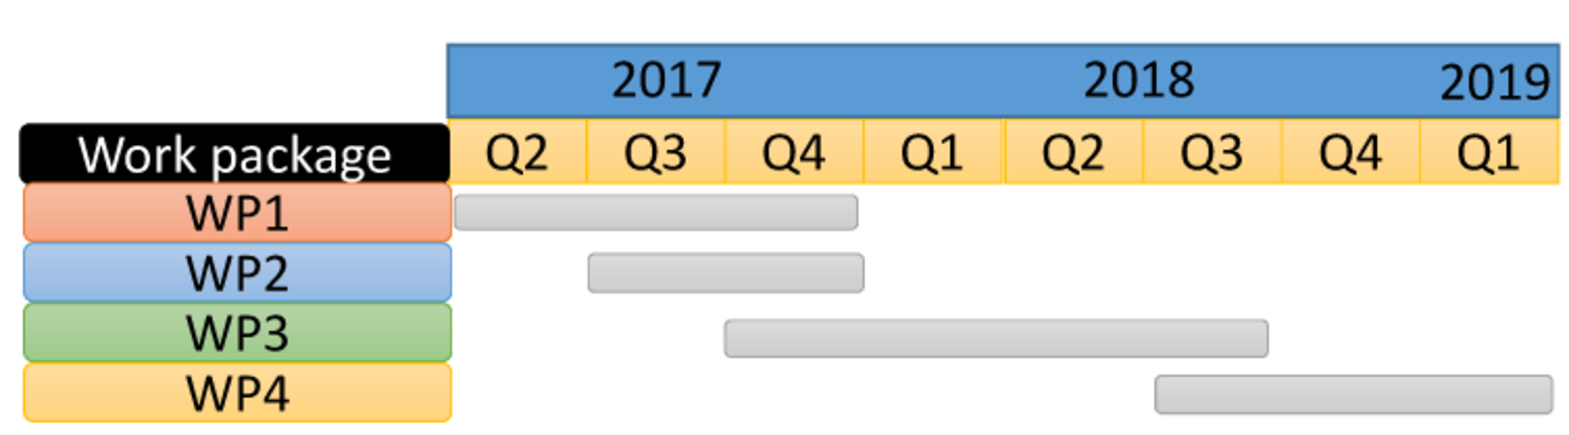
\includegraphics[width=8.0cm]{fig/Timeschedule.pdf}
%   \end{center}
    \caption{Time schedule for the project}
    \label{fig:schedule}
%     \vspace{-1.5cm}
\end{wrapfigure}
Optimization of a large environment such as a large telecommunications network requires the understanding of the data and computation.
When such an understanding is made, it is possible to implement actions that can optimize the computer system in the intended direction suggested by the company.
The following sections details the efforts for the project on optimization of mobile networks and Figure \ref{fig:schedule} illustrates the breakdown of the work packages on the timeline.
As seen in the figure, the main efforts for monitoring and analyzing Big Data is made is the early PoDoCo funded period, as well as a prototype implementation of the optimized network.
In the later phase, more elaborated optimization methods are being developed as well as real-time optimization methods.

\paragraph{WP1: Data monitoring}
The initial part of the project is to determine how to monitor the data stream.
Monitoring is required to collect the information in form of Big Data.
Radio access networks and mobile network is monitored for finding patterns of performance parameters like user experience or network faults. 
In this WP, we deploy monitoring features in the network or use log information to understand the past workload or data transfer imposed in the network.
At the end of this WP, we have gathered the main aspects of the network system of interest by the company.
Included in this WP is tool support for automatic monitoring based on the findings.
\paragraph{WP2: Data analysis}
WP2 covers appropriate methods to be applied on the collected data sample to filter out the interesting information.
The information gathered in this WP will represent, for example, the level of \textit{user satisfaction} or the \textit{performance} of the network system in place.
Based on the Big Data analysis, we suggest predictions methods that can represent the actual workload (or other desired property) to a close extent.
With network prediction methods in place, we can construct simulation environments, which later can be used to simulate an optimized network based on the findings in WP3 and WP4.
Our prediction methods are to be evaluated in terms of accuracy and performance in a real system environment.
\paragraph{WP3: Non real-time system optimization}
WP3 is about using the collected data in WP1 and the prediction methods in WP2 for building optimization methods in the telecommunications network.
The methods must include many-input, many-output optimization, which means that the design space is of considerable size.
We investigate several optimization methods like machine learning and regression models, and evaluate their accuracy both in simulation environments and in the real system.
Figure \ref{fig:schedule} shows an overlapping of WP1,2 and 3 at Q4 2017 because time to the process of monitoring and analyzing data must be allocated for allowing iterations for finding the data of interest.
Also creating simulation environments in WP2 might require input back from WP3.
In WP3, no real-time properties are considered which means that the computational overhead of the optimization algorithm is not considered.
The aim, in this WP, is to find accurate solutions rather than focusing on response time of the optimization solvers.
\paragraph{WP4: Real-time system optimization}
WP4 include similar characteristics as in WP3, but with a consideration on real-time processing.
In such an environment, there must be a fast enough response in the optimization algorithm in order to be useful.
Such restrictions usually bring a trade-off between accuracy and performance, and the best trade-off is to be selected in this WP.
WP4 is executed almost in sequence with no parallel WP since the data used in WP4 is most likely a simplified version of WP3 and no additional data from WP1 or WP2 is expected.

\section{Past experience}
The background of the PI is heavily influenced by achieving energy efficiency in multi-node/multi-core systems.
The thesis titled \textit{Energy Aware Software for Many-Core Systems} \cite{Holmbacka:15} was awarded with the grade of excellence and has been both a subject to a number of international cooperations in form of scientific articles and as practical use-cases like the freely available Android app ``Low Energy Player''\footnote{https://play.google.com/store/apps/details?id=org.videolan.vlc.LEL.lite.green\&hl=en}. \vspace{0.2cm}

The host university of the PI is currently leading a joint university project on Internet of Things called INTERSYS\footnote{http://iot4health.utu.fi/?p=374}.
We are developing methods to increase interoperability between nodes in IoT networks.
% The current problem within this domain is the very broad heterogeneity of both hardware and software, in other words, there are many standards for communication and it usually requires tailored software for handling the communication.
Our goal is to improve the ability for nodes of different vendors to communicate between and inside sensor networks.
As the network grow, the amount of data passing though the nodes becomes very large.
To enable an analysis of the data in more detail, we intend to allow applications express requirements more general and explicitly following the style of the work in \cite{Holmbacka:15},
such as CPU resources, bandwidth, throughput etc.
Self-aware applications in such networks increase the predictability of the workload because there is a level of insight into the application; it is not only a black box.
Self-aware software in network based systems allow an increased level of de-centralization (like in 5G), which means that decisions are made at the most appropriate location such as in the sensor itself, in the base station, in the fog or even in the cloud.
% It makes the network more ``living'' and allows a more scalable structure of intelligence.
Since the structure of IoT networks has similar characteristics as telecommunication networks, similar approaches might be feasible for such scenarios as well.
% The PI is directly involved in this project, and developing the general self-aware software is part of the post-doc research.
\vspace{0.2cm}

On a practical level we have been using machine learning for transcoding time prediction of online videos \cite{Deneke15}.
Machine learning is one tool to analyze large amounts of data with many parameters.
In this work, we predicted the transcoding time for online conversion of a collection of youtube video files to other formats based on support vector machines, linear regression and multi-layer perception feed forward artificial neural networks.
% The PI was not personally part of this particular work, but is closely working with the team developing the model.
\vspace{0.2cm}

A critical part of optimizing mobile networks is the ability to understand and predict the workload \cite{Zhu:08} applied on the system, for example in the network.
Predicting such a workload can solve overloading situations by balancing network streams onto many network nodes or improving the energy efficiency by shutting down (for the moment) unnecessary hardware.
Our current work in progress is a workload predictor for bursty-traffic video streaming networks proposed by a large Finnish telecommunications company.
In this work, we predict the processing time of jobs arriving on a bursty-traffic network, and our task is to develop a dynamic scalable system which is fast enough to handle the occasional high bursts of traffic and which is energy efficient enough to scale down resources when not needed.
The work is currently ongoing and a publication is expected in early 2017. \vspace{0.3cm}
% The PI is closely supporting the primary researcher, and the publication is being co-written by the PI.

\textit{My genuine interest for this project comes from my possibility of both integrating my mindset and skills in research in an industrial context but also from solving a practical problem for benefiting the industry. I also hope to bridge academia with the industry, and bring possibilities of cooperation in the future.}

\bibliographystyle{alpha}
{\footnotesize
\bibliography{sample}}

%----------------------------------------------------------------------------------------


\end{document}